\documentclass{llncs}
\usepackage{fixmetodonotes}
\usepackage[T1]{fontenc}
\usepackage[swedish]{babel}
\usepackage{graphicx}
\usepackage{pdfpages} 
\usepackage{listings}
\usepackage{color}
\usepackage{textcomp}
\usepackage{verbatim} 
\usepackage{minted}

\definecolor{javared}{rgb}{0.6,0,0} % for strings
\definecolor{javagreen}{rgb}{0.25,0.5,0.35} % comments
\definecolor{javapurple}{rgb}{0.5,0,0.35} % keywords
\definecolor{javadocblue}{rgb}{0.25,0.35,0.75} % javadoc

\lstset{language=PHP,
basicstyle=\ttfamily,
keywordstyle=\color{javapurple}\bfseries,
stringstyle=\color{javared},
commentstyle=\color{javagreen},
morecomment=[s][\color{javadocblue}]{/**}{*/},
columns=fixed,
numbers=left,
numberstyle=\tiny\color{black},
stepnumber=2,
numbersep=10pt,
tabsize=4,
 breaklines=true,
showspaces=false,
showstringspaces=false}
\usepackage[pdftex,bookmarks=true,bookmarksopen,bookmarksdepth=2]{hyperref}
\begin{document}
\hypersetup{
    bookmarks=true,         % show bookmarks bar?
    unicode=false,          % non-Latin characters in Acrobat?s bookmarks
    pdftoolbar=true,        % show Acrobat?s toolbar?
    pdfmenubar=true,        % show Acrobat?s menu?
    pdfnewwindow=true,      % links in new window
    hidelinks
}
\renewcommand\figurename{Figure}
\renewcommand\tablename{Table}
\renewcommand\listfigurename{Figures}
\renewcommand\listtablename{Tables}
\pagenumbering{arabic}
\title{PHP Framework Performance for Web Development}
%\titlerunning{PHP Framework Performance}  
% abbreviated title (for running head)
%                                     also used for the TOC unless
%                                     \toctitle is used
%
\author{H�kan Nyl�n}
%
%\authorrunning{H�kan Nyl�n}   % abbreviated author list (for running head)
%
%%%% list of authors for the TOC (use if author list has to be modified)
%\tocauthor{H�kan Nyl�n}
%
\institute{Blekinge Institute of Technology, Karlskrona, Sweden,\\
\email{hakan@dun.se}}

\date{21 March, 2012}

\maketitle
% A category with the (minimum) three required fields
%\category{H.4}{Information Systems Applications}{Miscellaneous}
%A category including the fourth, optional field follows...
%\category{D.2.8}{Software Engineering}{Metrics}[complexity measures, performance measures]

%\terms{Theory}
\renewcommand{\abstractname}{Abstract.}
\pagestyle {plain}
\begin{abstract}
{\bf [Context]} The new PHP Frameworks ideas has become popular for developers. 
It is also important to know how big impact they have on the performance. 
Bringing two top frameworks against each others can bring up some light how performance do look like today on the web with PHP as its grounds.  
{\bf [Problem]} Visitors have nowadays less energy to wait for a website to load. Meanwhile, PHP Framework has become known among developers, but you have been missing piece of performance that makes the load time to be reduced even more. so visitors can surf without any problems. Making it a good idea to try to discovery how the performance is on PHP Framework can change for a visitor.
{\bf [Contribution]} This paper is one of the first trying to perform performance experiments on PHP Frameworks.
It can help to push people to the right decisions in future work in PHP Framework Performance. 
The lack of data in this area is also one of the decision to make this paper as well.
\end{abstract}
\section{Introduction}
The World Wide Web, the internet started to be popular in the beginning of the 90s. 
The face towards the users was different websites, running on HTTP-servers, based on the official HTML language. 
And it began to be discussion about being able to store and perform calculations on data on websites, this was not possible to deal with static files like HTML was.
You could use several languages to do so, The Founder of PHP, Rasmus Lerdorf made PHP because of the massive amount of code you needed to code in PERL, a language PHP is based on,\cite{php:faq} to do a specific thing. It was as first only small PERL codes to make the coding more easier then before to code a website.
He created PHP just as it could handle the quest he needed to handle on his page. 
He released it just for fun and it became famous as a good idea to a simpler language for web development. 
Many join the project and it is now a big project, a script language that more and more become a more object-oriented script language. If not already.

The web is nowadays different. Many are talking about speed, speed and performance. 
For a website you have many different approaches to make the website faster, or you will lose visitors if the page load is too slow. 
A new service that came famous when cloud came the thing everyone should use, is CDN\footnote{CDN is Content Delivery Network, a network of servers. 
Where static data for websites and more can be stored, a CDN is spread all over the world, making the request faster.} and also different performance approaches, like the web-server, the server in general or the page. 
This could mean configuration or tweaks making the page load faster.

PHP Framework is mostly focused on fast development, with libraries and helpers, it can make the development of a website faster. 
This make it very popular among developers wanting to make a fast demo page for a new project. 
When the page is then up for production on a website, everyone can reach it.
This stage make it important to think about performance, because users is not waiting long to a page to load, like mostly did on the 90s because of the slow internet connection. 
PHP Framework make it fast for the developer but the point of the visitor is missing.

{\bf The research focus} will be to see how other evaluate web performance in general and to test the most used tool in those papers to evaluate two of the biggest PHP Frameworks, CodeIgniter and CakePHP.

{\bf The nature} of this thesis is define a good start how to think about performance of PHP Frameworks performance in specific and Web performance in general.

{\bf The expected outcome} of this thesis is to point to right direction when evaluate PHP Frameworks, the tests can been seen as a guideline for future work and as first attribution to get any real data of performance for PHP Frameworks. 

\section{The Background}
Evaluation is all about the performance. Performance in this paper is about load\footnote{loads means how long a request take, in milliseconds.}, but it can be hardware, network and more. 
Evaluation in general is how you can test the performance and in which way. 
This is very important in the choice of products nowadays.

The history starts when the PHP, PHP: Hypertext Preprocessor (recursive acronym), got born in 1995, 
Which only was a start. 
Now is PHP bigger and mainly a own ``programming language'', more called a script language \cite{php:faq}, for websites, inspired by java, C and PERL. \cite{php:faq} 
Developers using PHP has issues making good websites fast, so some developers started to developed PHP Frameworks to help to create better websites faster. 
There are two PHP Frameworks that has the most users, one is CodeIgniter  \cite{MVC:codeigniter}, that was first released 28 February 2006 \cite{php:codeigniter}. 
It is focused to great clean, fast framework for developers. 
The other Framework is CakePHP \cite{MVC:cakephp}, which was released in 2005. CakePHP is mainly inspired by Ruby on Rails. \cite{php:cakephp} 
\newpage
\subsection{MVC}
Model View Controller is a pattern to have 3 different types of classes, telling what they will do. \cite{MVC:phpTeam} 
Model will handle datahandling, like data from databases. 
View is the one that handle how the data should be shown for the client. 
Controller is the middle, collect data from model and making the data readable  and sending it to the view. 
This paper will be about testing the performance of CodeIgniter\cite{MVC:codeigniter} and CakePHP\cite{MVC:cakephp}.

A Example could be a news page. A user use a web browser to access the website, which connects to the controller seeing as point 1, in figure \ref{fig:mvcmodel}. Controller needs data from the database so it call a function in the model-class, seeing in point 2. The model is connecting the database and is handling the queries and is returning the data to the controller, as been seen on point 3. The controller is then getting the view, that is mostly contain the HTML and only use PHP to loop out the data, and gives the view the data to been shown, and return it to the user, seeing on point 4.
\begin{figure}[h]
\centering
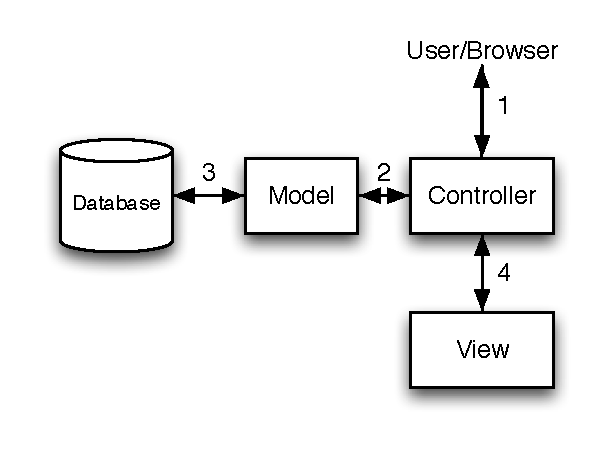
\includegraphics[scale=0.75]{mvc-diagram.eps}
\caption{A simple example how the structure for mvc could look like}
\label{fig:mvcmodel}
\end{figure}

\subsection{PHP Framework}
PHP is a server-side programming language famous to make it simple to develop in agile methods in web development. 
The Frameworks are based on MVC with add-ons, like form-helpers and database-controllers, in various languages, like PHP. 
Frameworks are built to make it even faster to develop a website. 
The biggest PHP Frameworks with MVC-thinking are CodeIgniter and CakePHP.

Codeigniter and CakePHP has many libraries to help the developer. 
Codeigniter has no official inspiration but its goal is to make it faster for the developer to create good websites then creating them from scratch in raw PHP. 
CakePHP is inspired by Ruby on Rails and you can see that on the structure of how you call the functions in a library in CakePHP. 
Codeigniter strongest ability is the openness where the developers are publishing libraries and plugins to Codeigniter.
 CakePHP has this ability too, but doesn't have as many followers making requests for changes in the code as Codeigniter.\footnote{This can be shown on their git repositories on Github, \cite{github:codeigniter} and \cite{github:cakephp}. 
 Seeing followers of the repository and how many pull requests each project has.}

The Difference is the structure but in the ground are both the same, 
they are based on MVC-thinking but over that, they both has difference structures and difference thinking how the libraries for databases and controllers, should behave and been called. 
The biggest difference was the handling the model. In CakePHP you only type the variables, which the model should handle from the database, normally. 
In Codeigniter you build the whole model with variables and own functions to get the data from the database. 
You can do that with CakePHP but by using the already implemented function to get, update, add and remove data from the table in the database.

\subsection{Client-side}
Client-side means the browser and the scripts and other rendering happening by the visitor on the site. 
This does have a big impact in the performance on a server. \cite{performance:Understanding} 
If using many images, the browser first loads the page and then send request to get the image and scripts on the page, adding more load to the server, 
because it generates more requests making the server handle more load. \cite{performance:dynweb}

\subsection{Server-side}
Server-side is the server. Here can the network, CPU and RAM be an impact in the performance for the visitor on the site. \cite{performance:dynweb} 
When Apache, the server software for web is getting many requests on the same time, more CPU and RAM will be used, making it to not handle all the requests when all RAM or CPU is used. 
Making the feeling of the website as slow. 
Often is the network that is stopping more load to the server, because the optimized server program such as Apache don not use so much of the CPU and RAM, making the CPU and RAM the less problem.

\subsection{Performance}
What performance can be different, to make it easy this paper will be about fast request, so network is very important. 
It can also have big impact how the servers is, Like a big server park in a data center. 
But that cost much money, which is a problem when doing this paper.
That is why it will only test this on cloud with one server and see how the framework is changing the ms of a request. 
This Server is running on Amazon EC2, an isolated server environment on the cloud. 
A good thing with this setup is that it is more or less this real website is set-up nowadays, making it more trustworthy in the data. 
The server specification can be seen on table \ref{table:serverSpecification}.


\section{Research}
\subsection{Research Questions}
\begin{description}
  \item[RQ1:] What web performance evaluations exist and how were they performed?
  \item[RQ2:] What factors impact web performance?\footnote{Because of the lack of data on php performance, it make it easier to find data about web performance in general.}
  \item[RQ3:] To what extent are open source php frameworks evaluated?
  \item[RQ4:] What performance are different between most commonly used open source php frameworks and how can it be evaluated?
\end{description}
Searched more or less on different types of strings like ``web development evaluation'' and ``Web development performance''. 
Found 300 papers and 8 relevant because the others was talking about the evaluation in general, not about performance in web development. 


\subsection{Research Methodology}
  \begin{tabular}{ l  r }
     
    Research Question & Methodology \\ 
    \hline
    RQ1 & Literature \\ 
    RQ2 & Literature \\
    RQ3 & Literature \\
    RQ4 & Data from RQ1, RQ2 and RQ3 to design experiment \\
  \end{tabular}
\subsection{Literature Survey}
The literature was found in different stages. And these sources was used.
\begin{itemize}
  \item Google Scholar
  \item IEEE
  \item Google
\end{itemize}

These strings were used, as seen in table \ref{table:literaturesearchstrings}.
\begin{table}[htbp]
\centering
\begin{tabular}{ p{6cm}}
  Strings\\
  \hline
  Web development Evaluation \\
  Web development Performance \\
  PHP Framework evaluation \\
  PHP Framework performance \\
  PHP Evaluation \\
  PHP Performance \\
  Website Performance \\
  Website evaluation \\
\end{tabular}
\caption[The strings for searching literature]{The strings for searching literature}
\label{table:literaturesearchstrings}
\end{table}

The selection was not so hard, Searched for some data that was doing something with evaluation in this area, and it was a few. 
The important was a good how-to, how they made the research to find out the information in the data, this was often found in the abstract but sometimes in the background. 
Often it was over 300 results in the search, but only 1-3 relevant pages, in every string, and the same papers was often in many of the strings.

\section{Literature review}
\subsection{The Approach}
The search was by the strings presented in Table \ref{table:literaturesearchstrings}, and by them the search found some hundreds of papers. 
This comes to the approach to found some with text such as impact in performance or was something about performance in PHP, because of the lack of papers in this area it become very hard to find any papers about PHP performance at all. This made it easier to find papers in web performance in general.
Took everything of value in this area, that have something that could be used for the questions to be answered such as impact in evaluation tests, php frameworks, different evaluation types and hows. 
The rest of the finding approach was depending on the authors knowledge, to find something that has an impact for a website or similar that can be an important thing to bring up in this paper.

\subsection{The Papers}
Information what the papers contains and what they have in common.
\subsubsection{PHP Team Development}
is about how the MVC idea and techniques make a difference in the development. 
This is a book about how the development in PHP is and what it does with web development, as MVC is a big part of it. This book is from 2009. \cite{MVC:phpTeam}

\subsubsection{Analysis of model-based mvc framework for php development CodeIgniter}
is analysing how the mvc based framework Codeigniter is doing in the development in performance and in userability for developers. 
this is an analysing paper from May 2009, it has kinda much in common with PHP Team Development, the book which have a chapter about MVC. \cite{MVC:codeigniter}

\subsubsection{Ec2 faq: What is an ec2 compute unit}
shows what EC2 is about and what a compute unit is. 
This is a website FAQ, which was last visited april 2012. \cite{EC2:Amazon}

\subsubsection{Understanding web performance}
presents how performance can be used and it is importance in the web business, it also bring up how performance can be tested and what can impact the tests. 
It is a paper presented in a Business Communication Review October 2001. \cite{performance:Understanding}

\subsubsection{A performance comparison of dynamic web technologies}
describe the different impact in performance when they do a comparison in different performance types and how it can be done. Presented in ACM Sigmetrics December 2003. \cite{performance:dynweb}

\subsubsection{Web-based IDE to create model and controller components for mvc-based web applications on cakephp}
writes how the CakePHP is build and how to code in it and talk a little about how MVC is about. A normal paper from December 2010. 
Has much in common with the other MVC framework Codeigniter and the book PHP Team Development. \cite{MVC:cakephp}


\section{Literature Results}
\subsection{Old Papers}
The results below are based on old papers. 
These papers are based on the general web performance and the web performance has not changed much in 10 years. 
The papers about web performance that is not 10 years old was very hard to find. 
They were mostly about java, an other programming language, that is not built up in the same way as php. Making them more or less useless for this paper. 
The papers bringed up in this paper are taking up impacts and other subject for the answers of the RQ, that has same impact and importance today. So the relevance has not changed.

\subsection{RQ1: What web performance evaluation exist and how were they performed?}
Evaluation in web is mostly done by load testing and counted in ms, but also in how to optimize the page itself to minimize request to server, like less pictures, or move them to another server. 
This can be seen in table \ref{table:rq1evaluation}.
\begin{table}[htbp]
\centering
\begin{tabular}{ p{4cm} p{3cm} p{2cm} }
  Evaluation topic & How & year\\
  \hline
  	requests/ms & Experiment & 2001\cite{performance:Understanding}\cite{performance:dynweb}\\
  	server/cpu & Experiment & 2003 \cite{performance:dynweb} \\
  	on-page optimization & Experiment & 2003\cite{performance:dynweb}\\
\end{tabular}
\caption[Different types of evaluation of a web performance]{Different types of evaluation of a web performance}
\label{table:rq1evaluation}
\end{table}

{\bf request/ms} is mostly used to evaluate performance of web applications. 
Got two different papers talking about two different things, \emph{Understanding Performance} adds this comment:
\begin{quote}
Sure, speed matters, but it is not a one-dimensional problem. 
And, despite what you have heard, just adding more bandwidth does not always make things go faster. \cite{performance:Understanding}
\end{quote}
Large and many requests needs good cpu and network, but to understand \emph{Understanding Performance} speed matters but not always the only problem. 
\emph{A Performance Comparison of Dynamic Web Technologies} talks about how they do the tests with requests in ms:
\begin{quote}
Consideration of overload behaviour may be just as important as the peak request rate when website administrators are choosing dynamic Web content generation technologies. \cite{performance:dynweb} 
\end{quote}
They saw an important to consider how to choose technologies using dynamic web content, because of different peak of request, making a need to handling the overload right. Something that can be changed in how many and how the size is on the requests. 
They also show how good it can be to evaluate how the performance is by using requests per milliseconds, or seconds.

{\bf server/cpu} is important when the server need to handle many requests at the same time. \emph{A Performance Comparison of Dynamic Web Technologies} tells that: 
\begin{quote}
Once the servers become overloaded, the CPU utilization of Apache 2.0.45 is lower than that of Apache 1.3.27. 
Under overload, Apache 2.0.45 is unable to accept TCP connections (and hence requests) as quickly as Apache 1.3.27. \cite{performance:dynweb}
\end{quote}
Making it important for cpu to work, but that does not mean that Apache itself make the CPU overload, it can be the network the cpu need to handle.

{\bf On-page optimization} is about how to create less requests to the server by removing or group images to one, because browsers loads the html first and then sending more request to get the images. 
This does also have a thing with the size of the images as well, Bigger images makes longer time to download. 
\emph{A Performance Comparison of Dynamic Web Technologies} is testing with static content \cite{performance:dynweb} that can be images or normal html files. Showing it goes faster than dynamic content, but it is a request.

\subsubsection{The pick}
will be to do request per ms in the tests, because the amount of papers already doing so, making it more trustworthy. The tests is to see any difference in the performance from visitors perspective, making it less important to evaluate server hardware and on-page optimization, even if the last one is interesting, we need to focus on one thing.
\newpage
\subsection{RQ2: What factors impact web performance?}
There are things that can be an impact of the performance while testing. The impacts are listed in table \ref{table:rq2evaluation}.
\begin{table}[htbp]
\centering
\begin{tabular}{ p{2cm} p{3cm} p{7cm} }
  Factor & How it impact & comment\\
  \hline
  	Server & network, cpu, ram & This can be fixed with a large server or a data center, something that can not be tested here.\\
  	\hline
  	Network & speed & if the test will do a request/ms load simulation, the network can be maximized without the server being touched to the performance limit which been set.\\
  	\hline
  	Wrong config & slowness, bad performance & wrong config on the server, resulting in less performance, but that will not be a problem. 
  	The default settings will be used. 
  	Change configuration for optimization is not a part of this paper.
\end{tabular}
\caption{Different types of evaluation of a web performance}
\label{table:rq2evaluation}
\end{table}

{\bf The server} can have big impact on performance because the cpu and RAM can be too less to handle the big amount of request tested. 
Small CPU and RAM can make it to overload in power and deny new request. 
Making it impossible to connect when that amount of request is full.

{\bf The Network} is not very important but the network should be stable for the amount of request sending to the server. 
Normal speed would be at least 10mbit down and 10mbit up to send and receive in good speed. 
The only problem with the network in my home is the stability, making it hard to trust the speed, making the ms higher than it should be. 
As example, the internet connection where the tests was tested can have 100mbit up and 100mbit down, but only getting 34 mbit of both because of the share of the internet connection, with 60 other people, this can be a big impact if all people is using the network, but that is not a big risk.

{\bf Wrong config} is the thing that can be spooky and many people do not know that it can be a default config or a wrong setup config that make the server to overload or not accept requests. 
The tests will use defaults just to make it so clean as possible, because that is how many people actually are using the defaults in the configs.

\subsubsection{The pick}
will be to trying to make it more realistic by using server on the cloud with good internet and good hardware.
\newpage
\subsection{RQ3: To what extent are open source php frameworks evaluated?}
Nothing was found that were about how performance in php framework evaluates. This could be as example that other authors probably think that this area is covered because of the performance papers in web generally. 
They are also outdated but it has not been any new invention in http performance neither. 
PHP is a script language making it totally different from normal web performance because of the compiling on hit, as we can call it. 
Meaning it runs through the PHP code when the file is called. 
Making a different in response, even if it is a little difference, almost not noticeable at all. 
And then add a PHP Framework on that. 
A difference in how you use php with libraries in a MVC maybe change the response time. 
This is why and what we will do in this paper.

\subsubsection{The pick}
will be to do this as a first step trying to perform a evaluation on PHP Framework, because of the lack of data.


\section{Experiment Design} 

\subsection{Investigated Question}
Which of the following php framework provide better performance measured in terms at: page speed in ms.

\subsection{Experiment artifacts and variables}


\subsubsection{Controlled Variables}
the following variables are controlled
\begin{table}[htbp]
\centering
\begin{tabular}{ p{3cm} p{7cm} }
  	Variable & Description\\
  	\hline
  	Request size & constant\\
  	Server & see table \ref{table:serverSpecification}\\
  	Framework & Compatible API, look at table \ref{table:classes} for info about the classes.\\
  	Response size & constant. See the size in table \ref{table:thedatafortests}.
\end{tabular}
\caption[Controlled variables in Experiment]{Controlled variables in Experiment}
\label{table:controlledvariables}
\end{table}

The tests is as you can see in the list below, all 3 tests will be run for database and without database, for each framework. Making it 6 tests total for a framework, with and without database.
\begin{table}[htbp]
\centering
\begin{tabular}{l l l l l l}
&\multicolumn{2}{l}{Codeigniter}&\multicolumn{2}{l}{CakePHP}\\
\cline{2-5}
 &Concurrency&Requests&Concurrency&Requests\\
 Test 1 & 5 & 20,000 & 5 & 20,000 & with database\\
 Test 2 & 5 & 20,000 & 5 & 20,000 & with database\\
 Test 3 & 5 & 20,000 & 5 & 20,000 & with database\\
 \hline
 Test 1 & 5 & 20,000 & 5 & 20,000 & withOUT database\\
 Test 2 & 5 & 20,000 & 5 & 20,000 & withOUT database\\
 Test 3 & 5 & 20,000 & 5 & 20,000 & withOUT database\\
\end{tabular}
\caption{How the tests will de done.}
\label{table:testsforframework}
\end{table}
the tests are using 5 for the concurrency level, meaning to send 5 requests each time, send so fast the previous requests are done. This to help to count the response time more exactly. You can see how the tests will be done in table \ref{table:testsforframework}.

The total amount of request of 20,000 is to get amount of request to get average time from, not too much and not too less. 
It does not need to be much more because the average will be the same $\pm$ 2 ms. 
That make it not necessary to have more. But it took as much as 20,000 because it make it more secure to be right numbers in the results.

A good thing to know is how the server will be setup, here is the table of the specification of the server that will be used for the experiment, on the Amazon cloud.
\begin{table}[htbp]
\centering
\begin{tabular}{ p{4cm}	 p{4cm} }
  System & Version/size \\
  \hline
  OS & Ubuntu 10.04 \\
  Apache & 2.2.14 \\
  MySQL & 5.4 \\
  PHP & 5.3.2 \\
  CPU & 1 EC2 Compute Unit\footnotemark[4] \\
  RAM & 1.7 GB \\
  HDD & 160 GB \\
  bits & 64 bits
\end{tabular}
\caption{The server specification where the test will be done on.}
\label{table:serverSpecification}
\end{table}
This is how the Framework classes will be used in the experiment.
\footnotetext[4]{One EC2 Compute Unit provides the equivalent CPU capacity of a 1.0-1.2 GHz 2007 Opteron or 2007 Xeon processor. \cite{EC2:Amazon}}
\begin{table}[htbp]
\centering
\begin{tabular}{ p{3cm} p{3cm} p{3cm} }
  Type & Codeigniter class & CakePHP class\\
  \hline
  	Controller & CI\_{}Controller & AppController\\
  	Model & CI\textunderscore{}Model & AppModel\\
	Database & database & database \\
	Form helper & form & Form\\
\end{tabular}
\caption{The different classes to use in the frameworks while coding a blog.}
\label{table:classes}
\end{table}
\subsubsection{Manipulated variables}
Server load measured in terms of amount of request.

Manipulated variables
\begin{description}
  \item[Response Type] HTML without database, HTML with database
\end{description}

Response Type is the only thing that will be changed. 
It is the support of the database that will be removed or added, making it possible to see the difference in performance for the core of the framework and for just the database controller.

\subsubsection{Experiment Artifact}
\begin{description}
  \item[blog] the blog will have normal features, or more likely very simple. It will have a normal list with pagination on the startpage, every post will have its own page. You can see the code in Appendix A1 and A3.
  \item[apache benchmark] will use Apaches own benchmark to simulate server load. 
  \item[Environment] the server is mostly already set, see table \ref{table:serverSpecification}.
\end{description}

{\bf Blog} is first a simple blog, with posts list on the start-page and with an own page for single post. 
The most important with the blog is the index page in the experiment, because it is there the requests will be send. 
Focusing to make a decent list of posts with title, body and created date at the blog. 
Both frameworks used the same database making it simple and less chance for the database to make a bad impact in the performance. 
You can see the code in Appendix A1 and A2.

{\bf Apache benchmark} is doing as All tools for performance for a web application is doing. 
It is same idea, to send an amount of request to the server and count how long it took to get a response back. 
Apache benchmark is the one that is been in while and has a reputation to do fair tests.\cite{apache:benchmark}

\section{Experiment}
\subsection{How it was made}
Used Apache benchmark to 20,000 requests on a currency of 5 request per time frame to a server. 
The test was made with a database randomly picked which framework to test. 
The tests without database other time, creating the difference on the ms.

I used the command line below to send the load request, randomly to specific ip-address\footnote[5]{the ip is typed as 11.11.11.11 to make it clear that the server is not running no more} on the day and night from my own computer to the test server, on the Amazon cloud on Ireland.
\begin{verbatim}
ab -wn 20000 -c 5 http://11.11.11.11/framework
\end{verbatim}

The variables controlled was response size, amount of request and currency of requests. 
see the data for the variables in table \ref{table:thedatafortests}.
\begin{table}[htbp]
\centering
\begin{tabular}{ p{2,6cm} p{2,5cm}  p{2,5cm}  p{2,3cm}  p{2,3cm} }
  {\bf Variable} & Codeigniter db\footnotemark[6] & Codeigniter & cakephp db\footnotemark[6] & cakephp \\
  \hline
  {\bf ResponseSize}\footnotemark[7] & 6440000 bytes & 6440000 bytes & 6360000 bytes & 6360000 bytes \\
  {\bf Requests} & 20,000 & 20,000 & 20,000 & 20,000 \\
  {\bf Currency} & 5 & 5 & 5 & 5 \\
\end{tabular}
\caption{The tests with database average request/connection times in ms.}
\label{table:thedatafortests}
\end{table}
\footnotetext[6]{with db it means database. In other meanings the framework with the database, the database was used with models for posts, without db it was just plain html in view with controller used.}
\footnotetext[7]{ResponseSize is total bytes of html sent from the server in one test, on every interval.}
\newpage
\subsection{The results}
The experiment was made randomly in different times, picked randomly. You can see how the tests was done in Table \ref{table:testsforframework}. The results of the tests can you see in Appendix A3.

The result can you see in figure \ref{fig:experimentwithdb}. 
It was almost same results on both, but a small gap between the two framework on just a few Millie seconds, to be exact, it was a gap on 5,34 ms in a average.
\begin{figure}[h]
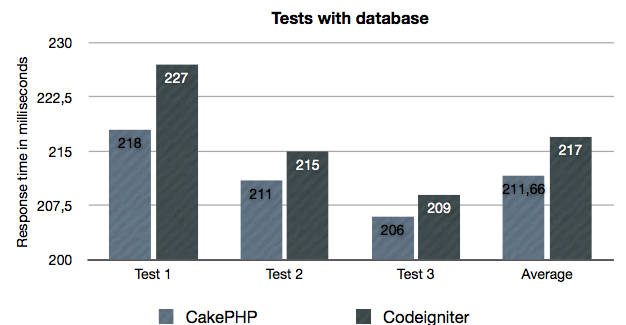
\includegraphics[scale=0.55]{charts-tests-database.png}
\caption{The tests with database average request/connection times in ms.}
\label{fig:experimentwithdb}
\end{figure}
\newpage
This was with database, with show that if we will focus to the ms total average, is CakePHP faster. This need to be tested without a database too, You can see the result in figure \ref{fig:experimentwithoutdb}.
\begin{figure}[h]
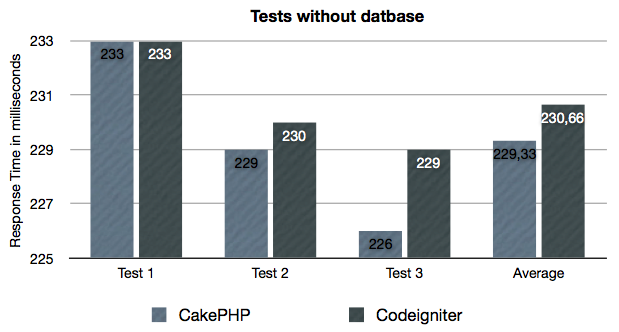
\includegraphics[scale=0.55]{charts-tests.png}
\caption{The tests without database average request/connection times in ms.}
\label{fig:experimentwithoutdb}
\end{figure}

The test without database shows that they are almost equally fast. Only 1,3 ms gap between them, CakePHP was faster here too, showing CakePHP has faster structure in its core.
\subsection{Data analysis and discuss}
This was good to  see how the different the performance is between the framework. 
This is also a very good way to evaluate the performance on any web service or application, the load of request can show how fast the request can be handled by the framework and show the fastness of it.

The biggest difference of the performance was when using a database, The difference was {\bf 5,34 ms}. It sounds little but in big sites just few ms does matter. 
The difference when using no database, only controller and view was no different, there was the difference {\bf 1,3 ms}. Very little. 
And if we bring the size in the thought, the gap is even lesser. 
Maybe is Codeigniter faster, if they was in same size? That can be true. 
The default template in CakePHP and Codeigniter was used, making the page in different sizes and could make a difference in the performance of the tests and request.

{\bf The difference in milliseconds} is so small without database because the frameworks seems to have good structure in their core of controllers and support for views, which we used in the tests without database for both framework. 
The difference in milliseconds for the tests with a database is bigger, 5.34 ms. Smaller than a thought but it is a difference. 
Making it noticeable when having a database and the PHP framework on a big website with many visitors. 
Creating a big queue of requests, making the small difference bigger, 5.34 ms can feel like the double, 10,68 ms or more. 
That is why a small difference can be important.

A thing to think about is the size difference, which was around {\bf 80,000 bytes}, for both the test with and without the database. 
This can make gap between the framework understandable with db, but without the db was the tests very close to each others. 
If the size was the same, Codeigniter could be faster. 

The difference in the size is because the use of the default in CakePHP and Codeigniter, CakePHP has more style and a usable template as default for the application, Codeigniter do not have it making it confused of the bigger size of the response. 
But the size is not a problem because of the choice to use the default of each framework, making the difference in the size.

This seems as no problem, used the default tools in both framework to make a very simple blog webpage. The size should in other word be different, it would be weird if it was not. 
But the thought that the size can make a difference is of course in the mind. 
It is request time in ms, and it does have a very big impact by the size.

Would love to see any {\bf future work} on different sizes for the PHP framework, which tests how the size does matter of the performance, with same size of both.

\subsection{Validity Threats}
\subsubsection{Tests are not isolated}
making the tests to be disturb by something from outside, can be the traffic of the line on Amazon cloud or something else that can make the response time longer or not trusted. 
This was tried to be reduced by been testing in the night. 
But you can see in the tests without, that was made more on the morning that the response time is already higher. 
This should not change the gap between the frameworks because all the tests was tested in the same time, making it having all around same response time in general. 

On other hand, a good thought would be that a good performance tests in a web perspective would be to have the webserver and the client on different locations, simulate real production website. Making it a more real data collected.

\subsubsection{Concurrency level} 
could be misunderstood which the low level, at 5.
A good thought is that the tests is meant to just test how the framework and PHP is handling in normally.
normally mean in this case 5 visitors at the same time.
This could be bigger or smaller. 
But these tests was not meant to see how the frameworks are handling the requests in high visitor numbers.


\subsubsection{Client's impact}
could be a problem. The tests were running Apache benchmark, but Apache benchmark is ignoring stylesheet and pictures (The blog in the test did not have pictures). 
It is just getting the generated html page, after php have generated it with the use of the code of PHP Framework. 
making the impact smaller than a normal browser, that is getting the stylesheet and pictures too.

\section{Conclusion}
The frameworks performance has big difference, but mostly just if in used of database, the classes fro using database can in other words be more effective. 
CakePHP was fastest in both tests, with and without a database. 
But the size was different on 80,000 bytes. 
This could be something that could make CakePHP a winner. 
But my conclusion is that used default template, very simple html page. So it does not have a big impact.

The fastest framework, according to the data is CakePHP, with just 1,3 ms without database and with 5,34 ms with database. 
This is something that is a big impact in the PHP performance and it can be fixed in newer versions. 

The experiment shows that the evaluation can be done it milliseconds for websites and web applications. 
With these data is the difference of evaluation between PHP framework not big at all, but it is a difference, even if it is a small one. 

The relevance and contribution of this paper is big because of the lack of papers and experiment made on PHP Frameworks. This is one of a new area of technology to test in performance.

Let the war begin between the php frameworks in performance.
\newpage
\listofnote
\renewcommand\refname{References}
\bibliographystyle{abbrv}
\bibliography{sigproc} 
\listofnote
\listoffigures
\listoftables
\newpage
\section*{Appendix}
\subsection*{A1. CodeIgniter Code}
controller/blog.php
\begin{minted}{php}
<?php
class Blog extends CI_Controller {
	public function __construct()
    {
        parent::__construct();
        $this->load->model('Posts_model', 'Posts', TRUE);
    }
    
    function index() {
    	$this->data->query = $this->Posts->getPosts(10, 0);
    	
    	$this->load->view('blog', $this->data);
    }
    
    function view($id) {
    	$this->data->query = $this->Posts->getPost($id);
    	$this->load->view('view', $this->data);
    }
}
?>
\end{minted}

view/blog.php
\begin{minted}{html}
<html>
<head>
<title>Le Blog</title>
<meta http-equiv="Content-Type" content="text/html; charset=utf-8" />
<link href="/codeigniter/css/cake.generic.css" rel="stylesheet">
<link href="/codeigniter/favicon.ico" type="image/x-icon" rel="icon" />
<link href="/codeigniter/favicon.ico" type="image/x-icon" rel="shortcut icon" />
</head>
<body>
<div style="hight:100px;font-size:18pt;font-family:helvetica,arial;width:100%">
<h1>My simple blog.</h1>
</div>

<div class="container">
<?
if($query->num_rows() > 0) {
	foreach ($query->result() as $row)
	{
		?>
		<div style="width:300px;font-size:8pt">
			<a href="blog/view/<?=$row->id?>">
				<h2><?=$row->title?></h2>
			</a>
		<p>Skrevs <?=$row->created?></p>
		<p><?=$row->body?></p>
		</div>
		<?
	}
}
else {
	?><p>No posts yet.</p><?
}
?>
</div>
</body>
</html>
\end{minted}

view/view.php
\begin{minted}{html}
<html>
<head>
<title>Le Blog</title>
<link href="/codeigniter/bootstrap/css/bootstrap.css" rel="stylesheet">
</head>
<body>
<div style="hight:100px;font-size:18pt;font-family:helvetica,arial;width:100%">
<h1>My simple blog.</h1>
</div>

<div class="container">
<?php
if($query->num_rows() > 0) {
$row = $query->row();
?>
<h2><?=$row->title?></h2>
<p>Created <?=$row->created?></p>
<p><?=$row->body?></p>
<?
}
?>
</div>
</body>
</html>
\end{minted}

model/posts\_{}model.php
\begin{minted}{php}
<?php
class Posts_model extends CI_Model {
	public $id = "";
	public $title = "";
	public $body = "";
	public $created = "";
	public $modified = "";
	
	function install()
	{
			/* First, create our posts table: */
		$this->db->query("CREATE TABLE posts (
    id INT UNSIGNED AUTO_INCREMENT PRIMARY KEY,
    title VARCHAR(50),
    body TEXT,
    created DATETIME DEFAULT NULL,
    modified DATETIME DEFAULT NULL
);");
	}
	
	function addPost($data) {
    	if($data) {
    		$this->db->insert('posts', $data); 
    	}
	}
	
	function getPosts($amount, $lastId = 0) {
		if($lastId == 0) {
			$data = $this->db->query("SELECT * FROM posts ORDER
			 BY ID DESC LIMIT 10");
		}
		else {
			$data = $this->db->query("SELECT * FROM posts WHERE id
			 <$lastId ORDER BY ID DESC LIMIT 10");
		}
		return $data;
	}
	
	function getPost($id = 0)
	{
		$data = "";
		if($id != 0) {
			$data = $this->db->query("SELECT * FROM posts
			 WHERE id ='{$id}' LIMIT 1");
		}
		return $data;
	}

}
?>
\end{minted}
\subsection*{A2. CakePHP Code}
controller/postsController.php
\begin{minted}{php}
<?php
class PostsController extends AppController {
    public $helpers = array('Html', 'Form');
    
    public function index() {
        $this->set('posts', $this->Post->find('all'));
    }
    
    public function view($id = null) {
    	$this->Post->id = $id;
        $this->set('post', $this->Post->read());
    }
}
?>
\end{minted}
view/posts/index.ctp
\begin{minted}{html}
<!-- File: /app/View/Posts/index.ctp -->

<h1>Blog posts</h1>
<table>
    <tr>
        <th>Id</th>
        <th>Title</th>
        <th>Created</th>
    </tr>

    <!-- Here is where we loop through our $posts array, printing out post info -->

<?php foreach ($posts as $post): ?>
    <tr>
        <td><?php echo $post['Post']['id']; ?></td>
        <td>
            <?php echo $this->Html->link($post['Post']['title'],
array('controller' => 'posts', 'action' => 'view', $post['Post']['id'])); ?>
        </td>
        <td><?php echo $post['Post']['created']; ?></td>
    </tr>
    <?php endforeach; ?>
    
</table>
\end{minted}
view/posts/view.ctp
\begin{minted}{html}

<!-- File: /app/View/Posts/view.ctp -->

<h1><?php echo h($post['Post']['title'])?></h1>

<p><small>Created: <?php echo $post['Post']['created']?></small></p>

<p><?php echo h($post['Post']['body'])?></p>
\end{minted}
model/Post.php
\begin{minted}{php}
<?php
class Post extends AppModel {
	public $validate = array(
        'title' => array(
            'rule' => 'notEmpty'
        ),
        'body' => array(
            'rule' => 'notEmpty'
        )
    );
}
?>
\end{minted}
\subsection*{A3. The Tests Results}
\includepdf[pages=-]{../experiment/tests.pdf} 
\newpage
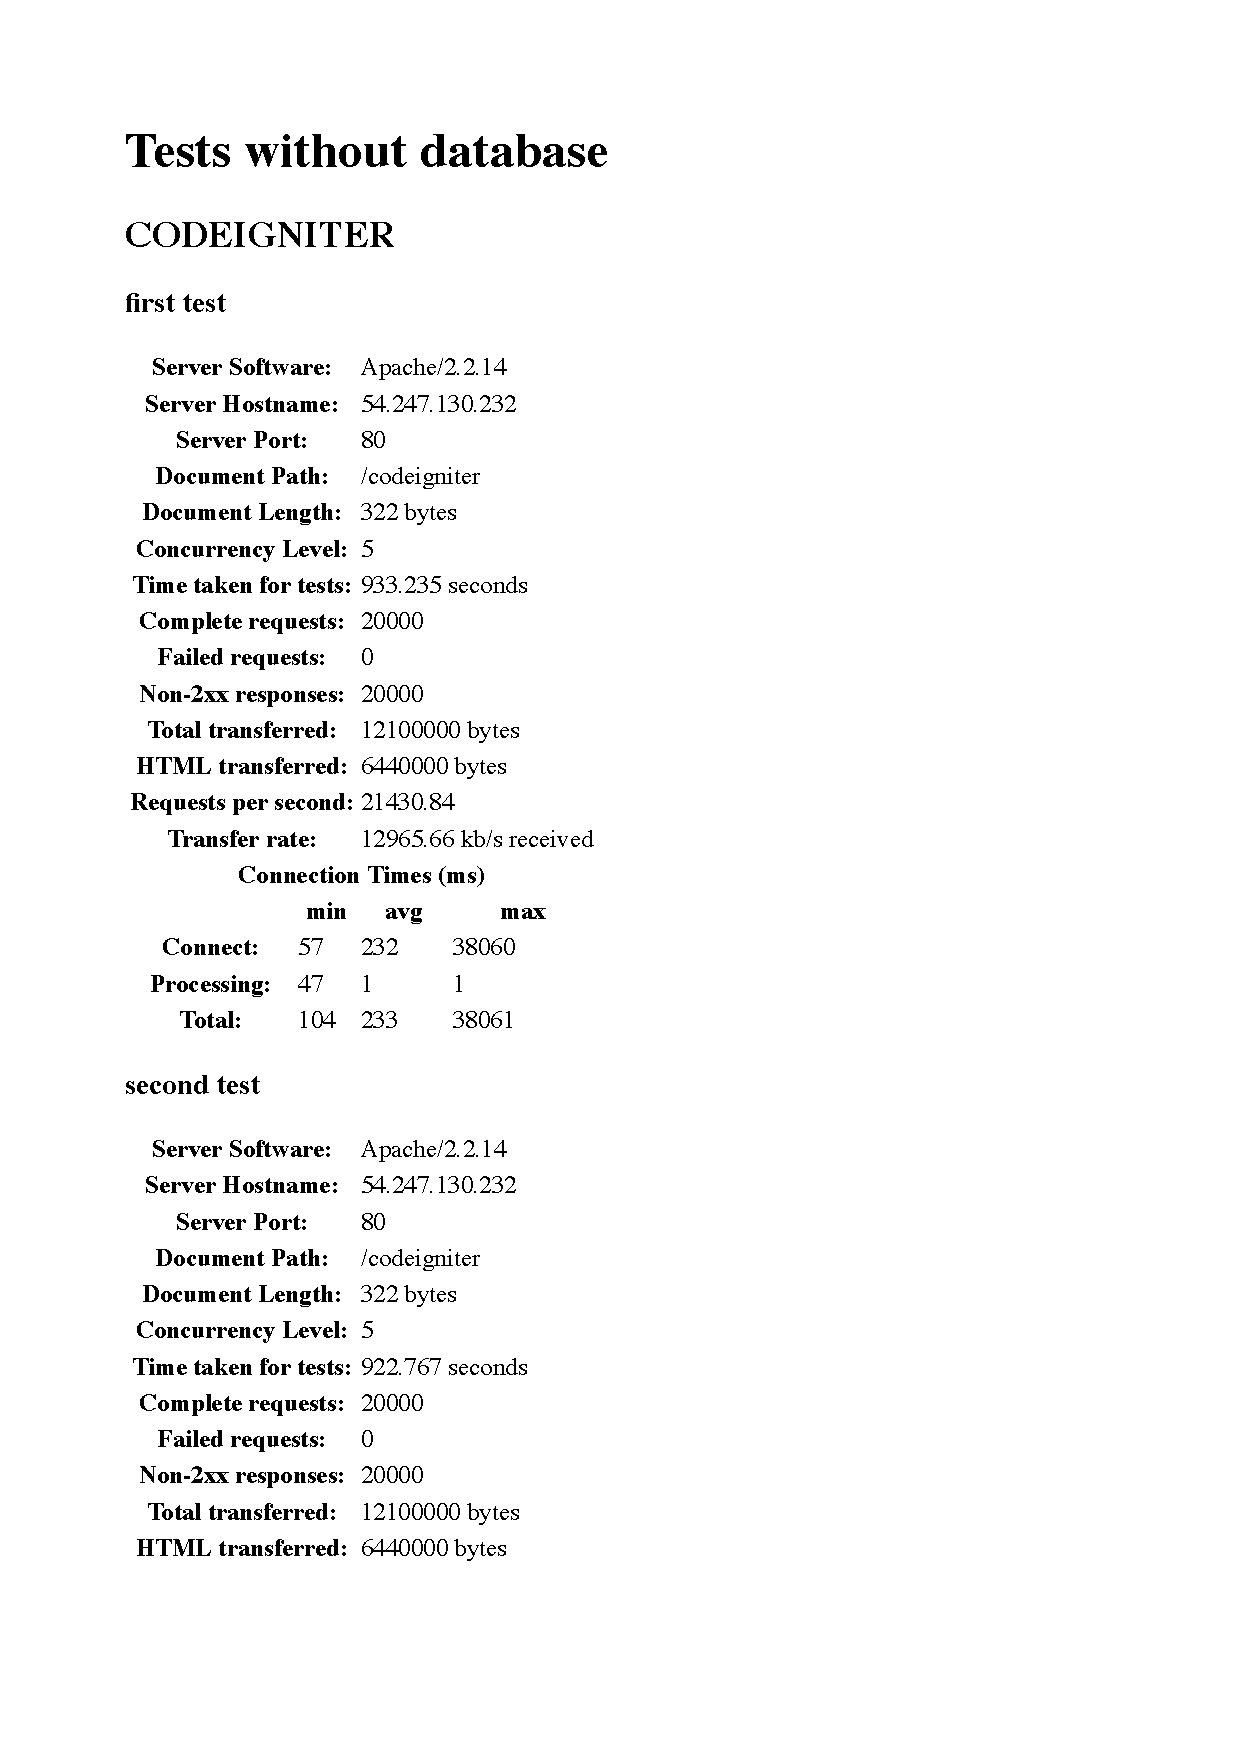
\includepdf[pages=-]{../experiment/testswithoutdb.pdf}
\end{document}
